\chapter[Referencial Teórico]{Referencial Teórico}
\label{refteorico}

\section{\textit{Shaders}: \textit{pipelines} programáveis}

	Conforme \cite{realtime}, \textit{shading} é o processo de utilizar uma equação para computar o comportamento da uma superfície de um objeto. Então, \textit{shaders} são algorítmos escritos pelo programador a fim de substituir as funcionalidades pré-definidas. Existem dois tipos de \textit{shader}, que focam diferentes partes do \textit{pipeline} gráfico: o \textit{vertex shader} e o \textit{fragment shader}. 

	O   \textit{vertex shader} é responsável pela manipulação dos dados dos vértices, incluindo coordenadas, normais, cores, sendo responsável pela alteração de posição e textura, por exemplo. Ele altera a etapa de \textit{vertex shading}, descrita na Seção \ref{renderpipe}. Ele deve, ao menos, definir as coordenadas de posição. 

	O \textit{fragment shader} opera nos fragmentos no processo de rasterização (selecionar e colorir os \textit{pixels}) antes de passar para a etapa de Fusão descrita na Seção \ref{renderpipe}, que faz as operações por fragmento (como o teste de profundidade). Ele deve, ao menos, atribuir uma cor para cada fragmento. 

	A linguagem GLSL (\textit{OpenGL Shading Language}) foi incluída na versão 2.0 da  \textit{OpenGL}, sendo desenvolvida com o intuito de dar aos programadores o controle de partes do processo de renderização (através dos \textit{shaders}), substituindo as funções fixas. A GLSL é baseada na linguagem C, mas antes de sua padronização o programador tinha que escrever o código na linguagem \textit{Assembly}, a fim de acessar os recursos da GPU. Além dos tipos clássicos do C, \textit{float}, \textit{int} e \textit{bool}, a GLSL possui outros tipos mostrados na Tabela \ref{tiposglsl}.

\begin{table}[h]
	\centering	
	\begin{tabularx}{0.9\textwidth}{cX}
		\toprule
		\textbf{Tipo} & \textbf{Descrição}  \\
		\midrule
		\texttt{vec2}, \texttt{vec3}, \texttt{vec4} & Vetores do tipo \textit{float} de 2, 3 e 4 entradas \\
		\texttt{ivec2},\texttt{ivec3}, \texttt{ivec4} & Vetores do tipo inteiro de 2, 3 e 4 entradas \\
		\texttt{mat2}, \texttt{mat3}, \texttt{mat4} & Matrizes 2x2, 3x3 e 4x4 \\
		\texttt{sampler1D}, \texttt{sampler2D}, \texttt{sampler3D} & Acesso a texturas \\
		\bottomrule
	\end{tabularx}
	\caption{ GLSL: tipos de dados}
	\label{tiposglsl}
\end{table}

	Além disso, a GLSL possui variáveis chamadas qualificadoras, que fazem o interfaceamento do programa e os \textit{shaders} e entre \textit{shaders}. Estas varáveis são mostradas na Tabela \ref{tiposqualificadores}.

	\begin{table}[h]
	\centering	
	\begin{tabularx}{0.9\textwidth}{cX}
		\toprule
		\textbf{Tipo} & \textbf{Descrição}  \\
		\midrule
		\texttt{attribute} &  Variável utilizada pelo programa para comunicar dados relacionados aos vértices para o \textit{vertex shader}\\
		\texttt{uniform} &  Variável utilizada pelo programa para comunicar dados relacionados com as primitivas para ambos os \textit{shaders} \\
		\texttt{varying} &  Variável utilizada pelo \textit{vertex shader} para se comunicar com o \textit{fragment shader} \\
		\bottomrule
	\end{tabularx}
	\caption{ GLSL: qualificadores}
	\label{tiposqualificadores}
	\end{table}

\section{Utilização de \textit{Shaders} em Plataformas Móveis}

	\subsection{Plataforma \textit{Android}}

	O \textit{Android} começou a ser desenvolvido em 2003 na empresa de mesmo nome, fundada por Andy Rubin, a qual foi adquirida em 2005 pela empresa \textit{Google}. A \textit{Google} criou a \textit{Open Handset Alliance}, que junta várias empresas da indústria das telecomunicações, como a \textit{Motorola} e a \textit{Samsung}, por exemplo. Assim, elas desenvolveram o \textit{Android} como é conhecido hoje, o qual é um sistema operacional  \textit{open source} para dispositivos móveis (baseado no \textit{kernel} do \textit{Linux}), tendo a primeira versão beta lançada em 2007 e segundo \cite{android2013}, hoje é o sistema operacional para \textit{mobile} mais utilizado.

	 Ainda de acordo com \cite{android2013}, em 2012 mais de 3,5 \textit{smartphones} com \textit{Android} eram enviados aos clientes para cada \textit{iPhone}. Em 2011, 500.000 novos \textit{devices} eram atividados a cada dia e em 2013, os números chegam a 1,5 milhões diários. O \textit{Android} também possui um mercado centralizado acessível por qualquer aparelho (\textit{tablet} ou \textit{smartphone}) chamado \textit{Google Play}, facilitando a publicação e aquisição de aplicativos. 
	O \textit{Android}  possui diferentes versões, sendo elas mostradas na Tabela \ref{androidTab} abaixo.  As versões mais novas possuem mais \textit{features} que as anteriores: a versão \textit{Jelly Bean}, por exemplo, possui busca por voz a qual não estava disponível na versão \textit{Ice Cream Sandwich}. 

\begin{table}[h]
	\centering	
	\begin{tabular}{cc}
		\toprule
		\textbf{Número da versão} & \textbf{Nome}  \\
		\midrule
		1.5 &  \textit{Cupcake} \\
		1.6 & \textit{Donut} \\
		2.0/2.1 &  \textit{Éclair} \\
		2.2 & \textit{FroYo} \\
		2.3 &  \textit{Gingerbread} \\
		3.0/3.1/3.2 & \textit{HoneyComb} \\
		4.0 & \textit{Ice Cream Sandwich} \\
		4.1/4.2/4.3 & \textit{Jelly Bean} \\
		4.4 &  \textit{KitKat} \\

		\bottomrule
	\end{tabular}
	\caption{ Versões da plataforma \textit{Android}}
	\label{androidTab}
\end{table}

	Uma das alternativas para o desenvolvimento em plataforma \textit{Android} é utilizar a ferramenta \textit{Eclipse}\footnote{http://www.eclipse.org/} (Figura \ref{eclipse}), que é um ambiente de desenvolvimento integrado (\textit{Integrated Development Environment} -- IDE) \textit{open source}. Adicionalmente, é preciso, de acordo com \cite{androidsdkmanager}, instalar o \textit{Android Software Development Kit}\footnote{http://developer.android.com/sdk/index.html} e o \textit{plugin} ADT (\textit{Android Development Tools})\footnote{http://developer.android.com/tools/sdk/eclipse-adt.html}, que permitem desenvolver e depurar aplicações pra \textit{Android}. Outra alternativa é utilizar o \textit{Android Studio}\footnote{http://developer.android.com/sdk/installing/studio.html}, lançado recentemente (2013) pela empresa \textit{Google}, que já vem com todos os pacotes e configurações necessárias para o desenvolvimento, incluindo o  \textit{Software Development Kit} (SDK), as ferramentas e os emuladores. 

	\begin{figure}[h]
	\centering
		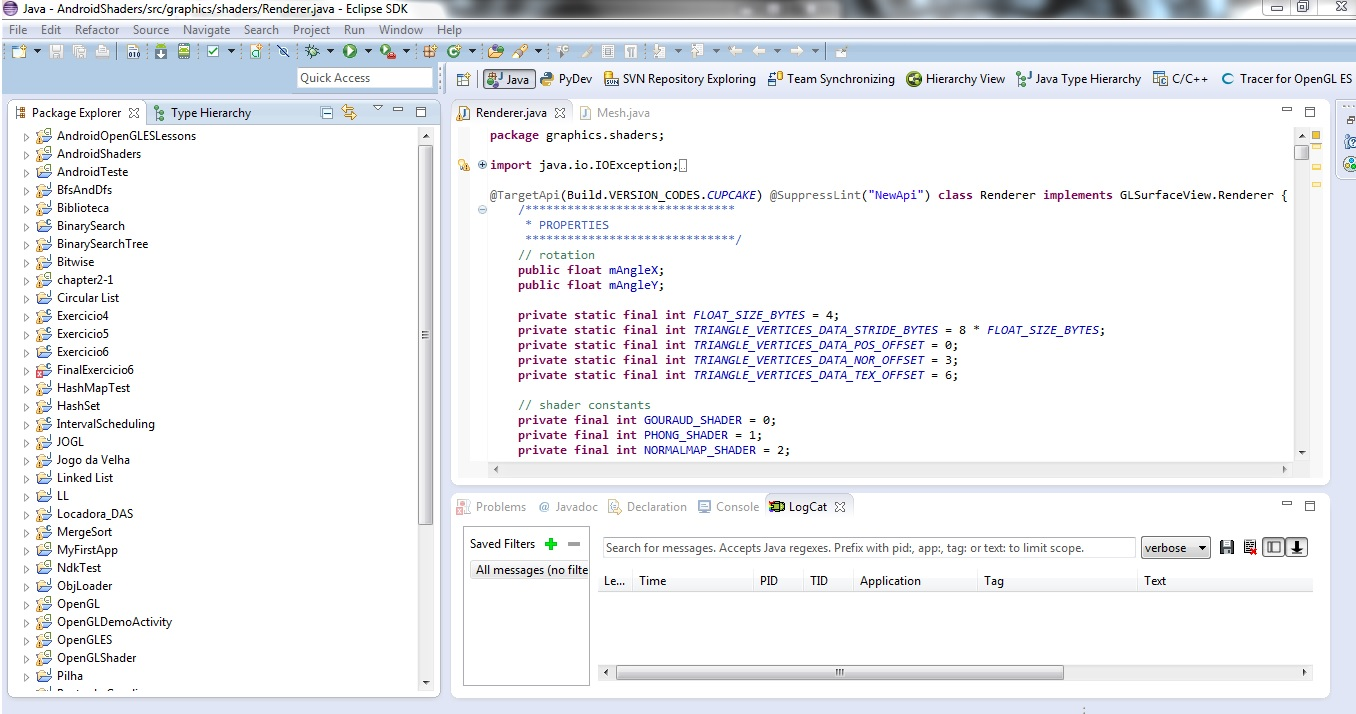
\includegraphics[keepaspectratio=true,scale=0.45]{figuras/eclipse.jpg}
	\caption{Ambiente de desenvolvimento \textit{Eclipse}}
	\label{eclipse}
	\end{figure}

	\subsection{\textit{OpenGL ES}}
	
	A \textit{OpenGL ES} (\textit{OpenGL for Embedded Systems}) foi lançada em 2003, e como citado em \cite{guha2011}, atualmente é uma das API's mais populares para programação de gráficos tridimensionais em pequenos \textit{devices}, sendo adotada por diversas plataformas como \textit{Android}, \textit{iOS}, Nintendo DS e \textit{Black Berry}. Segundo \cite{opengles2012}, ela possui três versõe: a 1.x que utiliza as funções fixas de renderização, a 2.x, que elimina as funções fixas e foca nos processos de renderização manipulados por \textit{pipelines} programáveis e a 3.x, que é completamente compatível com a  \textit{OpenGL} 4.3.  

	\subsubsection{\textit{Pipeline de Renderização}}
\label{renderpipe}


	O processo de geração de gráficos tridimensionais em computadores tem início com a criação de cenas. Uma cena é composta por objetos, que por sua vez são compostos por primitvas geométricas (como triângulos, quadrados, linhas, entre outros) que são constituídas de vértices, estabelecendo a geometria. Todos estes vértices seguem um processo similar de processamento para formarem uma imagem na tela.  Este processo pode ser divido em dois subprocessos principais: o de geometria e o de rasterização.  Segundo \cite{realtime}, o processo de geometria pode ser divido nas etapas mostradas na Figura \ref{geometria}.

	\begin{figure}[h]
	\centering
		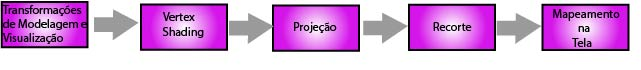
\includegraphics[keepaspectratio=true,scale=0.7]{figuras/geometria.jpg}
	\caption{Etapas do subprocesso de geometria}
	\label{geometria}
	\end{figure}

	Na etapa Transformações de Modelagem e Visualização, as coordenadas do objeto são transformadas, de forma que ele possa ser posicionado, orientado e tenha um tamanho determinado. Após o ajuste das coordenadas, é dito que o objeto está localizado no espaço do mundo e, em seguida, é aplicada a transformação de visualização, que tem como objetivo estabelecer a câmera na origem, mirando em direção ao eixo z negativo. 

	A próxima etapa é a de \textit{Vertex Shading}, responsável por modelar parte dos efeitos (a outra parte é feita durante a rasterização), pois renderizar somente a forma e posição não é suficiente.  Estes efeitos incluem as características dos materiais atribuídos aos objetos, como também os efeitos da luz, sendo que cada efeito pode ser modelados de diferentes formas, como representações de descrições físicas. Muitos dados são armazenados em cada vértice, como a sua localização e e o vetor normal associado (que indica a orientação do vértice no espaço), por exemplo. Assim, os resultados do \textit{vertex shading} são mandados para o subprocesso de rasterização para serem interpolados. 

	A etapa de projeção é responsável por transformar o volume de visualização aplicando métodos de projeção, como a perspectiva e a ortográfica (também chamada de paralela). A projeção ortográfica resulta em uma caixa retangular, em que linhas paralelas permanecem paralelas após a transformação. Na perspectiva, quanto mais longe um objeto se encontra, menor ele aparecerá após a projeção: linhas paralelas tendem a convergir no horizonte. Ela resulta em um tronco de pirâmide com base retangular. 

	Somente as primitivas gráficas que se encontram dentro do volume de visualização que serão renderizadas. Assim, o recorte (chamado \textit{clipping}) é responsável por não passar adiante as primitivas que se encontram fora da visualização. Primitivas que estão parcialmente dentro são recortadas, ou seja, o vértice que está de fora não é renderizado e é substituído por um novo vértice (dentro do volume de visualização). A  Figura \ref{clip} mostra esta ideia.

       \begin{figure}[h]
       \centering
	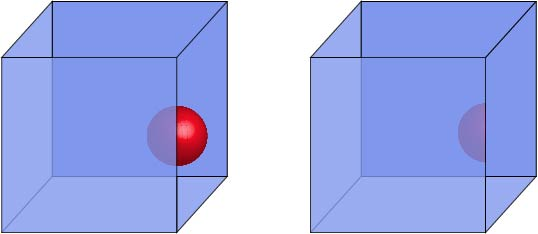
\includegraphics[keepaspectratio=true,scale=0.8]{figuras/clip.jpg}
       \caption{Antes do recorte (cubo de visualização esquerdo) e depois do recorte (cubo de visualização direito)}
       \label{clip}
       \end{figure}


	A última etapa de geometria é a de Mapeamento na Tela, cuja entrada é formada pelas primitivas recortadas e as coordenadas ainda tridimensionais. Assim, esta etapa tem como finalidade mapear as coordenadas tridimensionais em coordenadas de tela. Para isto, o centro de um \textit{pixel} (\textit{picture element}) é igual a coordenada 0,5. Então, \textit{pixels} de [0; 9] equivalem à cobertura das coordenadas de [0,0; 10,0). E os valores dos \textit{pixels} crescem da esquerda para a direita e de cima para baixo.

	Terminado o processo de geometria, o próximo a ser feito é o de rasterização, em que seu objetivo é computar e definir as cores para cada \textit{pixel}. Este processo pode ser dividido nas quatro etapas mostradas na Figura \ref{rasteriza}.

   \begin{figure}[h]
       \centering
	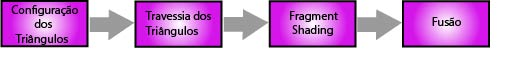
\includegraphics[keepaspectratio=true,scale=0.8]{figuras/rasteriza.jpg}
       \caption{Etapas do processo de rasterização}
       \label{rasteriza}
       \end{figure}

	Na etapa de Configuração dos Triângulos, dados são computados para as superfícies dos triângulos. Eles serão utilizados para a conversão dos dados vindos do processo de geometria (coordenadas e informações provenientes do \textit{vertex shader}) em \textit{pixels} na tela e também para o processo de interpolação. 

	A Travessia de Triângulos checa se cada um dos \textit{pixels} está dentro de um triângulo ou não. Para cada \textit{pixel} que sobrepõe um triângulo, um fragmento é gerado, conforme mostrado na Figura \ref{traversal}. Cada fragmento tem informações sobre sua localização na tela, no triângulo e sua profundidade, e as propriedades dos fragmentos dos triângulos são geradas usando dados interpolados entre os três vértices do triângulo. 

  \begin{figure}[h]
       \centering
	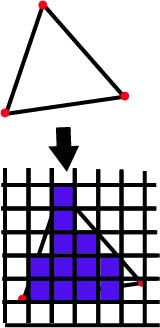
\includegraphics[keepaspectratio=true,scale=0.8]{figuras/traversal.jpg}
       \caption{Travessia de triângulos: fragmentos sendo gerados}
       \label{traversal}
       \end{figure}

	As computações por \textit{pixel} são calculadas durante o \textit{Fragment Shading}, em que o resultado consiste em uma ou mais cores a serem passadas para o próximo estagio. Muitas técnicas podem ser aplicadas durante esta etapa, e uma das mais importantes é a de texturização (que aplica no fragmento do objeto parte de uma imagem). 

	 A informação relacionada com cada \textit{pixel} é armazenada no \textit{color buffer}, que é um \textit{array} de cores. Assim, a última etapa é a de fusão, que é responsável por combinar a cor do fragmento gerada pelo estágio anterior com a cor armazenada no \textit{buffer}. Ela também é responsável pela visibilidade, em que o \textit{color buffer} deve conter as cores das primitivas da cena que são visíveis do ponto de vista da câmera. Isto é feito através do Z-\textit{buffer} (também chamado de \textit{buffer} de profundidade), que para cada \textit{pixel} armazena a coordenada $z$ a partir da câmera até a primitiva mais próxima.  Então, a coordenada $z$ de uma primitiva que está sendo computada é comparada com  o valor do Z-\textit{buffer} para o mesmo \textit{pixel}. Se o valor for menor, quer dizer que a primitiva esta mais próxima da câmera do que o valor da anterior, e assim, o valor do Z-\textit{buffer} é atualizado para o atual. Se o valor corrente for maior, então o valor do Z-\textit{buffer} não é modificado. 


\section{Teoria Matemática para Implementação de \textit{Shaders}}

	\subsection{Equação de Iluminação de \textit{Phong}}
	\label{flatgouphon}

	Na área de computação gráfica, os {\textit{Flat Shading}, \textit{Gouraud Shading} e \textit{Phong Shading} (compostos pelos \textit{vertex} e \textit{fragment shaders}) são um dos \textit{shaders} mais conhecidos. No método \textit{Flat Shading}, renderiza-se cada polígono de um objeto com base no ângulo entre a normal da superfície e a direção da luz. Mesmo se as cores se diferenciem nos vértices de um mesmo polígono, somente uma cor é escolhida entre elas e é aplicada em toda o polígono.  

	A computação dos cálculos de luz nos  vértices seguida por uma interpolação linear do resultado é conhecida como \textit{Gouraud Shading} (considerada superior ao \textit{Flat Shading}, pois renderiza uma superfície mais suave, lisa), criada por Henri Gouraud, sendo conhecida como avaliação por vértice. Nela, o \textit{vertex shader} deve calcular a intensidade em cada vértice e os resultados serão interpolados. Em seguida, o \textit{fragment shader} pega este valor e passa adiante. Segundo  \cite{guha2011}, é o padrão implementado pela  \textit{OpenGL}. 

	No \textit{Phong Shading}, primeiramente interpolam-se os valores das normais das primitivas e então computam-se os cálculos de luz para cada \textit{pixel}, utilizando as normais interpoladas. Este método também é conhecido como avaliação por \textit{pixel}. A intensidade de luz é calculada de acordo com a equação de luz de \textit{Phong} mostrada em \cite{guha2011}.

	 A \textit{OpenGL} oferece este tipo de \textit{shading} como opção, embora o mesmo possa ser implementado utilizando \textit{shaders}.  Ele requer maior poder de processamento do que a técnica \textit{Gouraud Shading}, pois cálculos nos vértices são computacionalmente menos intensos comparados aos cálculos feitos por \textit{pixels}. Porém, a desvantagém da técnica de \textit{Gouraud Shading} é que efeitos de luz que não afetam um vértice de uma superfície não surtirão efeito como, por exemplo, efeitos de luz localizados no meio de um polígono não serão renderizados corretamente. Porém, se o efeito ocorrer em um vértice, o \textit{Phong Shading} renderiza corretamente o vértice, mas irá interpolar erroneamente. A Figura \ref{fgp} mostra a diferença entre as três técnicas de \textit{shading} aplicadas em uma esfera com uma luz direcional. 

	\begin{figure}[h]
	\centering
		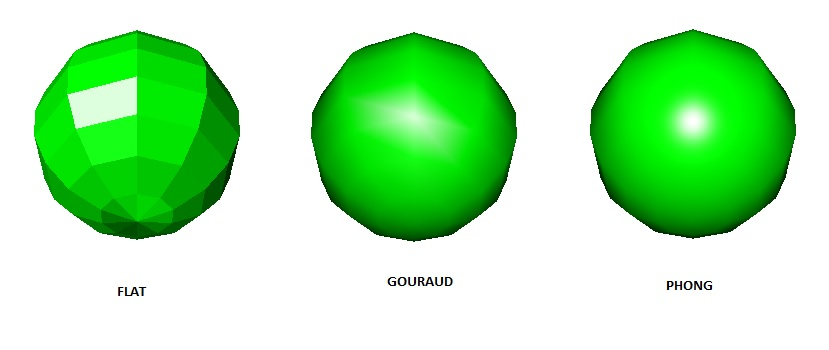
\includegraphics[keepaspectratio=true,scale=0.5]{figuras/flatgp.jpg}
	\caption{Comparação entre as técnicas de \textit{shading}}
	\label{fgp}
	\end{figure}

	\subsection{Renderização de Efeito \textit{Cartoon}}

	\subsection{Renderização de Efeito de Reflexão}
		\subsubsection{Conceitos de Álgebra Linear Utilizados}

\section{Complexidade Algorítmica Calculada de Forma Empírica}

	\subsection{Complexidade Algorítmica - Teoria}

	Complexidade algorítmica é uma medida que compara a eficiência de um determinado algorítmo, analisando o quão custoso ele é (em termos de tempo, memória, custo ou processamento). Ela foi desenvolvida por Juris Hartmanis e Richard E. Stearns no ano de 1965. Segundo \cite{complexidade}, para não depender do sistema em que está sendo rodado e nem da linguagem de programação, a complexidade algoritmica se baseia em uma função (medida lógica) que expressa uma relação entre a quantidade de dados e de tempo necessário para processá-los.

	 Como o cálculo visa a modelagem do comportamento do desempenho do algorítmo a medida que o número de dados aumenta, os termos que não afetam a ordem de magnitude são eliminados, gerando a aproximação denominada complexidade assintótica. Assim, a  Equação (\ref{compl1}) poderia ser aproximada pela  Equação (\ref{compl2})

	\begin{equation}
		y = n^{2} +10 n + 1000
	\label{compl1}
	\end{equation}

	\begin{equation}
		y \approx  n^{2} 
	\label{compl2}
	\end{equation}

	A maioria dos algorítmos possui um parâmetro $n$ (o número de dados a serem processados), que afeta mais significativamente o tempo de execução. De acordo com \cite{complexidade2}, a maioria dos algorítmos se enquadram nos tempos de execução proporcionais aos valores da Tabela \ref{complexidadeAlgoritmica}.

\begin{table}[h]
	\centering	
	\begin{tabularx}{0.9\textwidth}{cX}
		\toprule
		\textbf{Complexidade} & \textbf{Descrição}  \\
		\midrule
		Constante &  Ocorre quando as instruções do programa são executadas apenas uma vez.\\
		log N & Ocorre geralmente em programas que resolvem grandes problemas dividindo-os em partes menores, cortando o seu tamanho por uma constante.  \\
		N & Ocorre quando o programa é linear, ou seja, o  processamento é feito para cada elemento de entrada. \\
		$ N log N$ & Ocorre quando o problema é quebrado em partes menores, sendo resolvidas independentemente, e depois suas soluções são combinadas \\
		$ N^{2}$ & Ocorre quando o algorítmo é quadrático, ou seja, quando processa todos os pares de itens de dados. \\
		$ N^{3}$ & Ocorre quando o algorítmo é cúbico, ou seja, quando processa todos as triplas de itens de dados. \\
		$ 2^{N}$ & Ocorre quando o algorítmo segue uma função exponencial, ou seja, quando o N dobra o tempo de execução vai ao quadrado. \\
	
		\bottomrule
	\end{tabularx}
	\caption{ Valores mais comuns de complexidade algorítmica}
	\label{complexidadeAlgoritmica}
\end{table}


	\subsection{Métodos dos Mínimos Quadrados}
	\label{metminqua}

	O método dos mínimos quadrados é utilizado para ajustar pontos $(x,y)$ determinados experimentalmente a uma curva. No caso do ajuste a uma reta (dada por $y = a + bx$) muitas vezes estes pontos não são colineares e segundo \cite{minq} é impossível encontrar coeficientes $a$ e $b$ que satisfaçam o sistema.

	 Então, as distâncias destes valores para a reta podem ser consideradas como medidas de erro e os pontos são minimizados pelo mesmo vetor (minimizando a soma dos quadrados destes erros).  Assim, existe um ajuste linear de mínimos quadrados aos dados, e a sua solução é dada pela Equação (\ref{minquad}), em que é possível determinar os coeficientes $a$ e $b$ e consequentemente, a equação da reta. 

	\begin{equation}
		v =( M^{T}M)^{-1}M^{T}y
	\label{minquad}
	\end{equation}
	onde
	\begin{equation}
	M = \left[\begin{array}{cc}
               	1 & x1 \\
               	1 & x2  \\
		. & .  \\
               	. & .  \\
		1 & xn
          	         \end{array}\right] \mbox{,} \quad
	v = \left[\begin{array}{c}
               	a \\
               	b  
          	         \end{array}\right] \mbox{e} \quad
	y = \left[\begin{array}{c}
               	y1 \\
               	y2  \\
		.   \\
               	.   \\
		yn
          	         \end{array}\right] 	
	\label{variaveis}
	\end{equation}

	De acordo com \cite{calculo}, a função da exponencial pode ser dada como na Equação (\ref{expo}), em que $e$, $c$, $k$ são constantes ($e$ é a constante neperiana).  

	\begin{equation}
	\label{expo}
		y = ce^{-kt}
	\end{equation}

	Aplicando a função logarítimo dos dois lados da equação, obtém-se a  Equação (\ref{expo2})

	\begin{equation}
	\label{expo2}
		\ln{y} = \ln{c}  + \ln{e^{-kt}}
	\end{equation}
 	que pode ser simplificada na  Equação (\ref{eqn03}) (em que $b$ é uma nova constante) que equivale à equação da reta. 

	\begin{equation}
	\label{eqn03}
		\bar{y} = \bar{a} + \bar{b}t
	\end{equation}	

	Assim, é possível aplicar os métodos dos mínimos quadrados descritos anteriormente, aplicando o logaritmo nos dois lados da equação da exponencial. Os novos valores de $M$ e $y$ passam a ser: 

	\begin{equation}
	M = \left[\begin{array}{cc}
               	1 &  \ln{x1} \\
               	1 & \ln{x2}  \\
		. & .  \\
               	. & .  \\
		1 & \ln{xn}
          	         \end{array}\right] \mbox{,} \quad
	y = \left[\begin{array}{c}
               	\ln{y1} \\
               	\ln{y2}  \\
		.   \\
               	.   \\
		\ln{yn}
          	         \end{array}\right] 
	\label{nvar}
	\end{equation}

	O valores finais dos coeficientes $\bar{a}$ e $\bar{b}$ determinam os parâmetros c e k da exponecial através das relações

	\begin{equation}
	c = e^{\bar{a}}\, \, \, \mbox{e}\, \, \,\bar{b} = -k
	\end{equation} 


\subsection{Formato \textit{obj}}
\label{formatobj}

	Em uma cena, os modelos tridimensionais podem variar muito mais do que formas básicas como uma esfera e um torus, por exemplo. Assim, o formato \textit{obj} foi criado pela empresa  \textit{Wavefront} e é um arquivo para leitura de objetos tridimensionais, a fim de carregar geometrias mais complexas. Segundo \cite{graphicsprog}, neste arquivo cada linha contém informações a respeito do modelo, começando com uma palavra-chave, seguida da informação. A  Tabela \ref{palavraschave} mostra as principais palavras-chave utilizadas. 

\begin{table}[h]
	\centering	
	\begin{tabular}{cl}
		\toprule
		\textbf{Palavra-chave} & \textbf{Significado}  \\
		\midrule
		\texttt{usemtl} & Indica se está utilizando material  \\
		\texttt{mtlib} &  Nome do material \\
		\texttt{v} &  Coordenadas x, y e z do vértice \\
		\texttt{vn} & Coordenadas da normal \\
		\texttt{vt} &  Coordenadas da textura \\
		\texttt{f} &  Face do polígono \\
		\bottomrule
	\end{tabular}
	\caption{ Palavras-chave do formato obj}
	\label{palavraschave}
\end{table}

	A face do polígono (f) possui três índices que indicam os vértices do triângulo. Assim, cada vértice possui um índice (que depende de quando ele foi declarado), começando a partir de um. A Figura \ref{objFile} mostra o exemplo de um arquivo obj para a leitura de um cubo. 

	\begin{figure}[h]
	\centering
		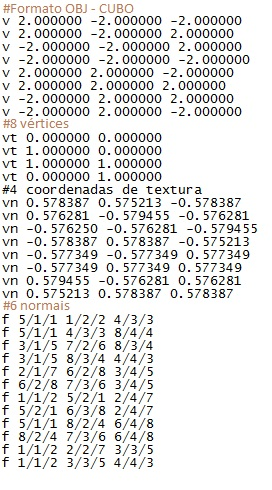
\includegraphics[keepaspectratio=true,scale=0.9]{figuras/obj.jpg}
	\caption{Arquivo \textit{obj} de um cubo}
	\label{objFile}
	\end{figure}

	Então, a partir da leitura do arquivo  \textit{obj}, é possível ler cada linha e armazenar em estruturas de dados as informações que serão passadas para renderizar o modelo tridimensional, como vértices e índices, e utilizar um dos métodos apresentados anteriormente para renderizar a cena. 
